\begin{frame}
    \centering
    \textbf{\Large{Poisson operator}}
\end{frame}

\begin{frame}
    \frametitle{Non-standard operator representation}
    \scriptsize
    \begin{columns}
    \begin{column}[b]{0.6\linewidth}
    \begin{itemize}
	\item	The multiwavelet basis is well suited for\\ 
        \textbf{integral convolution operators}
	    \begin{equation}
		\nonumber
		g(\boldsymbol{r}) = \left[T f\right](\boldsymbol{r}) = 
		    \int K(\boldsymbol{r} - \boldsymbol{r'})f(\boldsymbol{r'}) d\boldsymbol{r'}
	    \end{equation}
        \pause
	\item \textbf{Scaling projection} of operator at scale $n$
	    \begin{equation}
		\nonumber
		T \approx T^n
	    \end{equation}
        \pause
	\item \textbf{Wavelet projections} by differences
	    \begin{equation}
		\nonumber
		T^{n+1} - T^n = A^n + B^n + C^n
	    \end{equation}
        \pause\pause\pause\pause
	\item \textbf{Multiresolution operator} by recursion
	    \begin{equation}
		\nonumber
		T^N = T^0 + \sum_{n=0}^{N-1} \left[A^n + B^n + C^n\right]
	    \end{equation}
	%\item Scaling operator $T$ is \textbf{dense}
	%\item Wavelet operators $A$, $B$ and $C$ are \textbf{sparse} 
    \end{itemize}
    \end{column}
    \begin{column}[b]{0.4\linewidth}
    \begin{center}
    \only<2>{\hspace{4.0mm}
        
\includegraphics[scale=0.6, clip, viewport = 240 280 450 480] {figures/matrix/matrix_1.pdf}
        \vspace{15mm}
    }
    \only<3>{\hspace{3.4mm}
        
\includegraphics[scale=0.6, clip, viewport = 240 280 450 480] {figures/matrix/matrix_2.pdf}
        \vspace{15mm}
    }
    \only<4>{\hspace{2.8mm}
        
\includegraphics[scale=0.6, clip, viewport = 240 280 450 480] {figures/matrix/matrix_3.pdf}
        \vspace{15mm}
    }
    \only<5>{\hspace{2.2mm}
        
\includegraphics[scale=0.6, clip, viewport = 240 280 450 480] {figures/matrix/matrix_4.pdf}
        \vspace{15mm}
    }
    \only<6>{\hspace{1.6mm}
        
\includegraphics[scale=0.6, clip, viewport = 240 280 450 480] {figures/matrix/matrix_5.pdf}
        \vspace{15mm}
    }
    \only<7>{\hspace{1mm}
        
\includegraphics[scale=0.6, clip, viewport = 240 280 450 480] {figures/matrix/matrix_6.pdf}
        \vspace{15mm}
    }
    \only<8>{
        \textbf{Poisson kernel}
        \begin{equation}
	    \nonumber
	    P(\boldsymbol{r}-\boldsymbol{r}') = 
	    \frac{1}{4\pi}\ \frac{1}{|\boldsymbol{r}-\boldsymbol{r}'|}
        \end{equation}

        \vspace{15mm}

        \textbf{Helmholtz kernel}
        \begin{equation}
	    \nonumber
	    H^{\mu}(\boldsymbol{r}-\boldsymbol{r}') = \frac{1}{4\pi}\ 
	    \frac{e^{-\mu |\boldsymbol{r}-\boldsymbol{r}'|}}
            {|\boldsymbol{r}-\boldsymbol{r}'|}
        \end{equation}
        \vspace{15mm}

        \tiny
        G. Beylkin, R. Coifman, V. Rokhlin, \\
        {\it Commun. Pure Appl. Math.}
        \textbf{44(2)}
        (1991)
    }
    \end{center}
    \end{column}
    \end{columns}
\end{frame}

\begin{frame}
    \frametitle{Vanishing moments}
    \scriptsize
    \centering
    \textbf{A function $f$ has $M$ vanishing moments if}
    \begin{equation}
        \nonumber
        \mu_m = \int_0^1 x^m f(x) dx = 0,\qquad m = 0, 1, \dots, M - 1
    \end{equation}
    \vspace{2mm}
    \begin{itemize}
        \item   Scaling basis has no vanishing moments $\longrightarrow$ 
		\textbf{long ranged} interaction
        \item   Wavelet basis has $k$ vanishing moments $\longrightarrow$ 
		\textbf{short ranged} interaction
    \end{itemize}
    \vspace{2mm}
    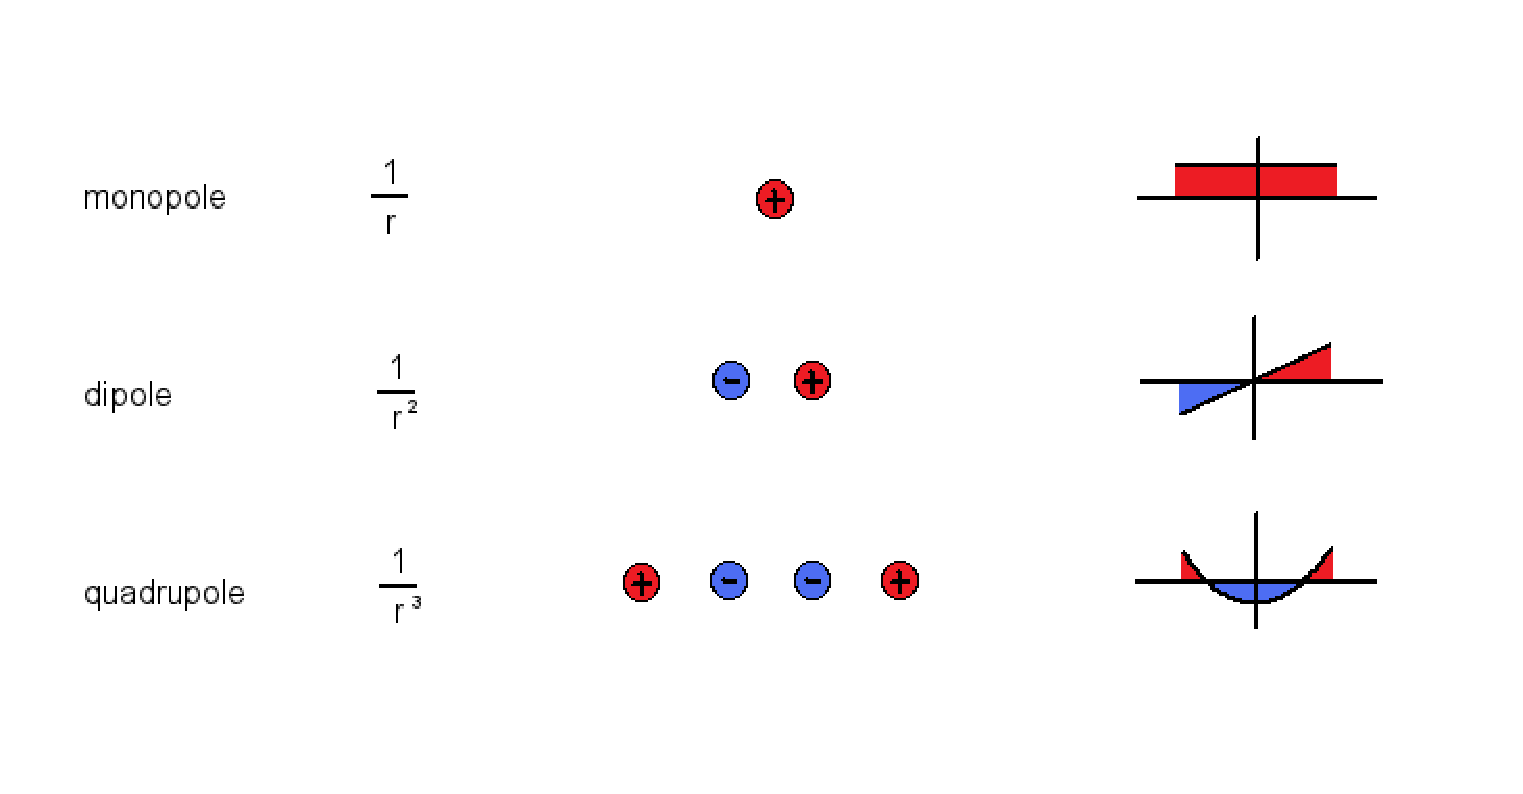
\includegraphics[scale=0.4, clip, viewport = 0 50 680 350]{figures/multipoles.pdf}
\end{frame}

\begin{frame}
    \frametitle{Coulomb interaction}
    \scriptsize
    \begin{itemize}
	\item	Electrostatic potential from a \textbf{charge density} is given by the Poisson equation
		\begin{equation}
		    \nonumber
		    -\nabla^2 V(\boldsymbol{r}) = \rho(\boldsymbol{r})
		\end{equation}
		\vspace{2mm}
	\item	Can be solved directly in integral form using the Poisson kernel
		\begin{equation}
		    \nonumber
		    V(\boldsymbol{r}) = 
		    \int P(\boldsymbol{r}-\boldsymbol{r'})\rho(\boldsymbol{r'}) d\boldsymbol{r'} =
		    \int\frac{\rho(\boldsymbol{r'})}{4\pi|\boldsymbol{r} - \boldsymbol{r'}|} d\boldsymbol{r'} 
		\end{equation}
		\vspace{2mm}
    \end{itemize}
    \pause
    \begin{columns}
    \begin{column}{.30\textwidth}
    \end{column}
    \begin{column}{.40\textwidth}
        \ \ \ \ \textbf{Numerical problems}
        \begin{itemize}
	    \item Not Cartesian separable
	    \item Singularity at short-range
	    \item Slow decay at long-range
	\end{itemize}
    \end{column}
    \begin{column}{.30\textwidth}
    \end{column}
    \end{columns}
\end{frame}

\begin{frame}
    \frametitle{Separation of variables using Gaussians}
    \scriptsize
%    \centering
%    The Poisson equation is solved in integral form using the Poisson kernel
%    \begin{equation}
%	\nonumber
%	V(\boldsymbol{r}) = \int P(\boldsymbol{r}-\boldsymbol{r'})
%        \rho(\boldsymbol{r'}) d\boldsymbol{r'} =
%	\int\frac{\rho(\boldsymbol{r'})}
%        {4\pi|\boldsymbol{r} - \boldsymbol{r'}|} d\boldsymbol{r'} 
%    \end{equation}

%    \vspace{3mm}

    \begin{columns}
    \begin{column}{.56\textwidth}
    \begin{itemize}
	\item The Poisson kernel can be approximated
	    \begin{equation}
		\nonumber
		\frac{1}{\boldsymbol{r}} \approx 
                \sum_{i=1}^M a_i e^{-\alpha_i \boldsymbol{r}^2} 
	    \end{equation}
	\item Any accuracy can in principle be obtained
	\item Full operator is decomposed into $M$ terms
	\item Each operator term is applied separately
    \end{itemize}

    \vspace{6mm}

    \pause\pause\pause\pause\pause\pause\pause
    \hspace{3mm} \textbf{Solves numerical problems}
    \begin{itemize}
	\item	Separates coordinates
	\item	Removes singularity
	\item	Separates length scales
    \end{itemize}

    \end{column}
    \begin{column}{.45\textwidth}
	\only<1>{\hspace{2mm}
        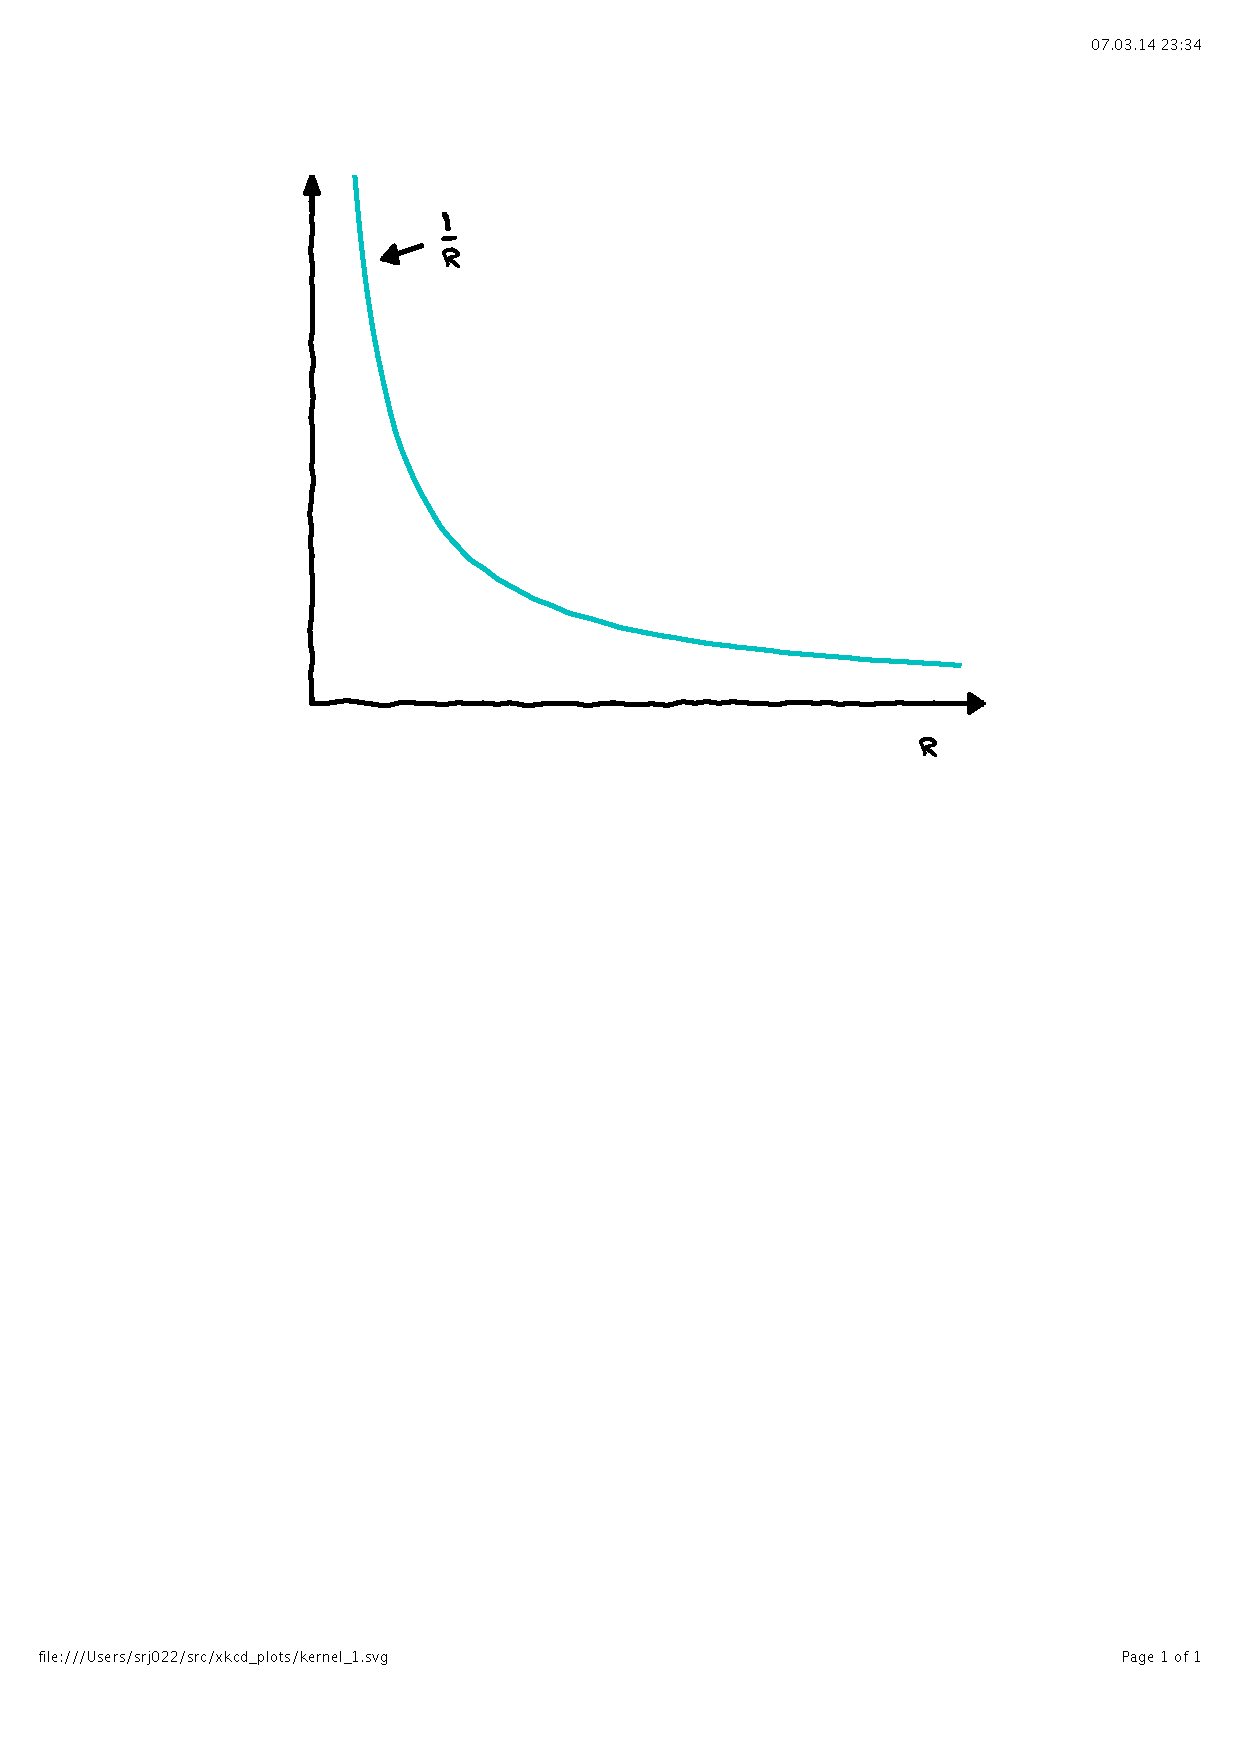
\includegraphics[scale=0.4, clip, viewport = 110 450 490 800] {figures/kernel_1.pdf}}
	\only<2>{\hspace{2mm}
        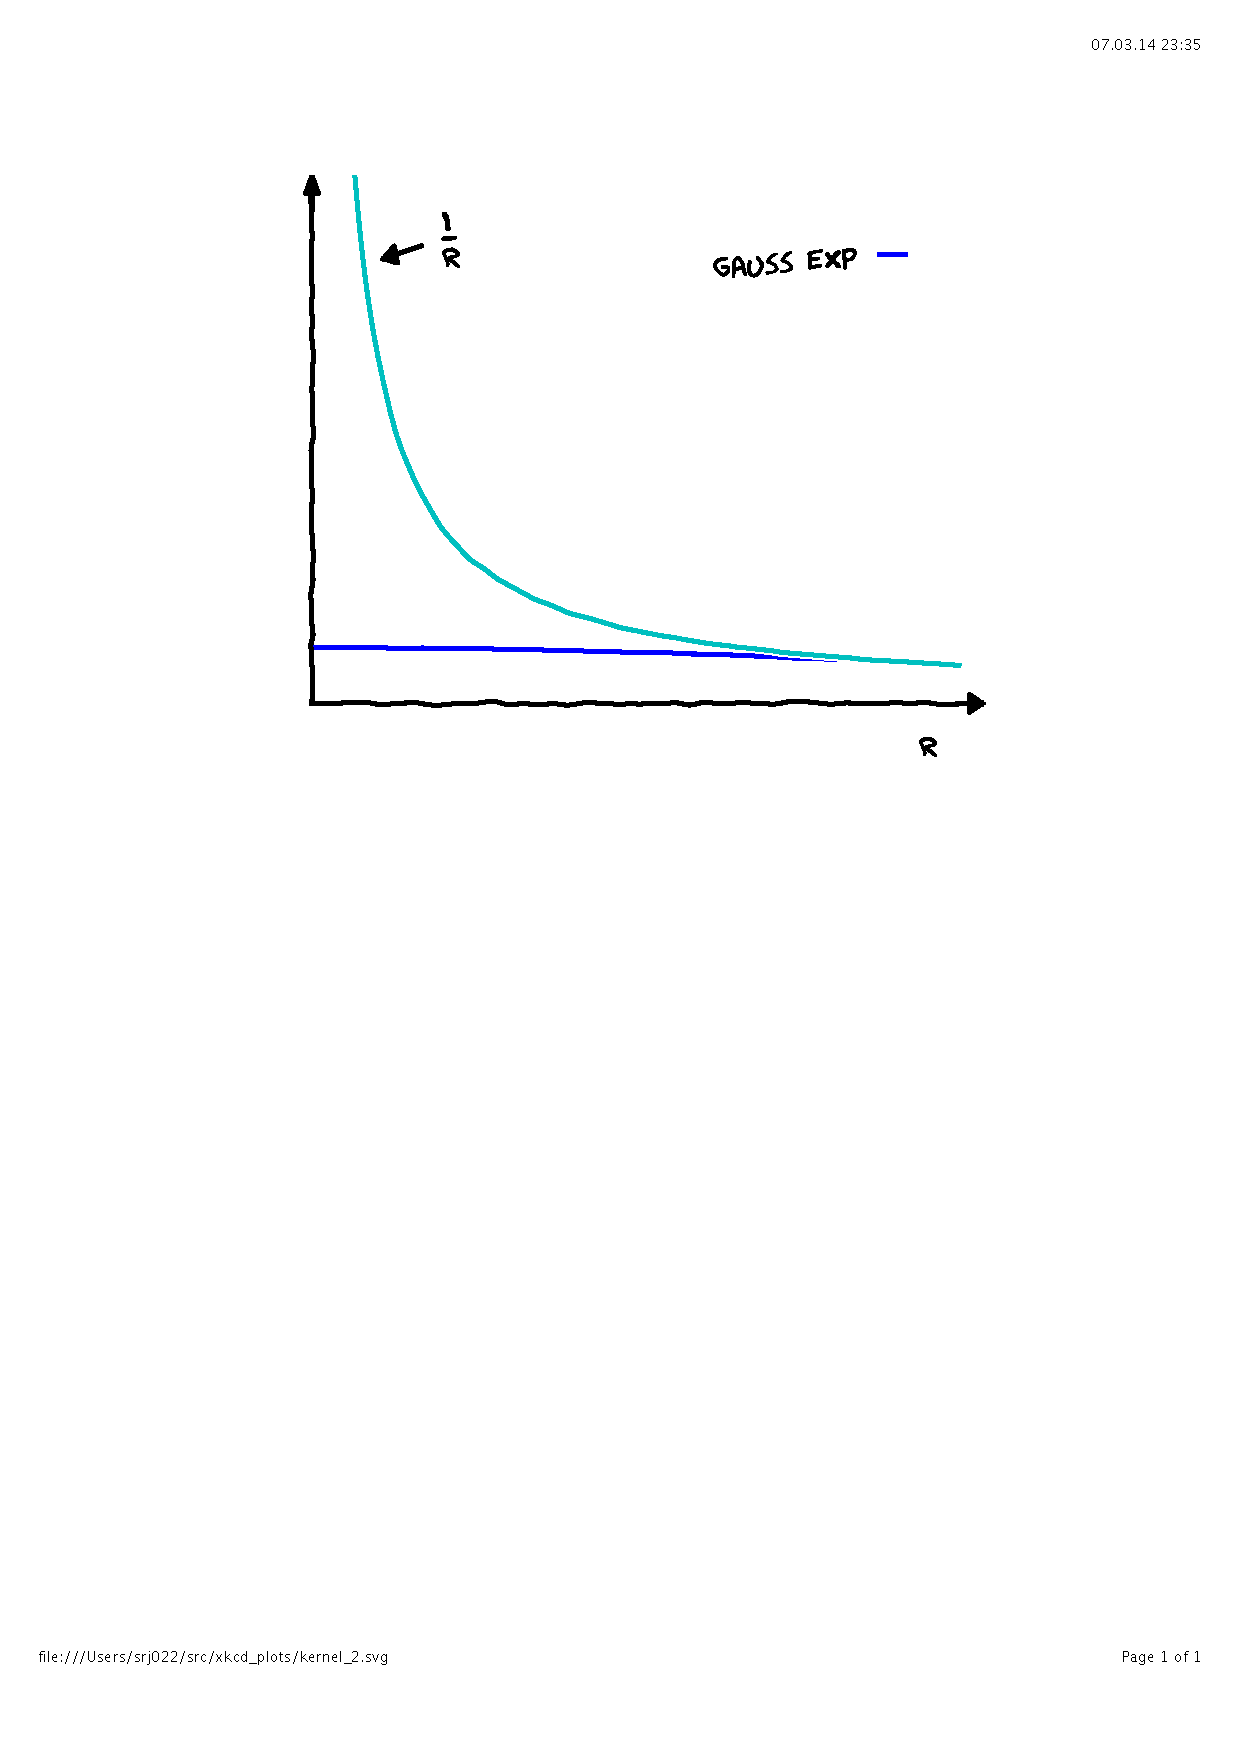
\includegraphics[scale=0.4, clip, viewport = 110 450 490 800] {figures/kernel_2.pdf}}
	\only<3>{\hspace{2mm}
        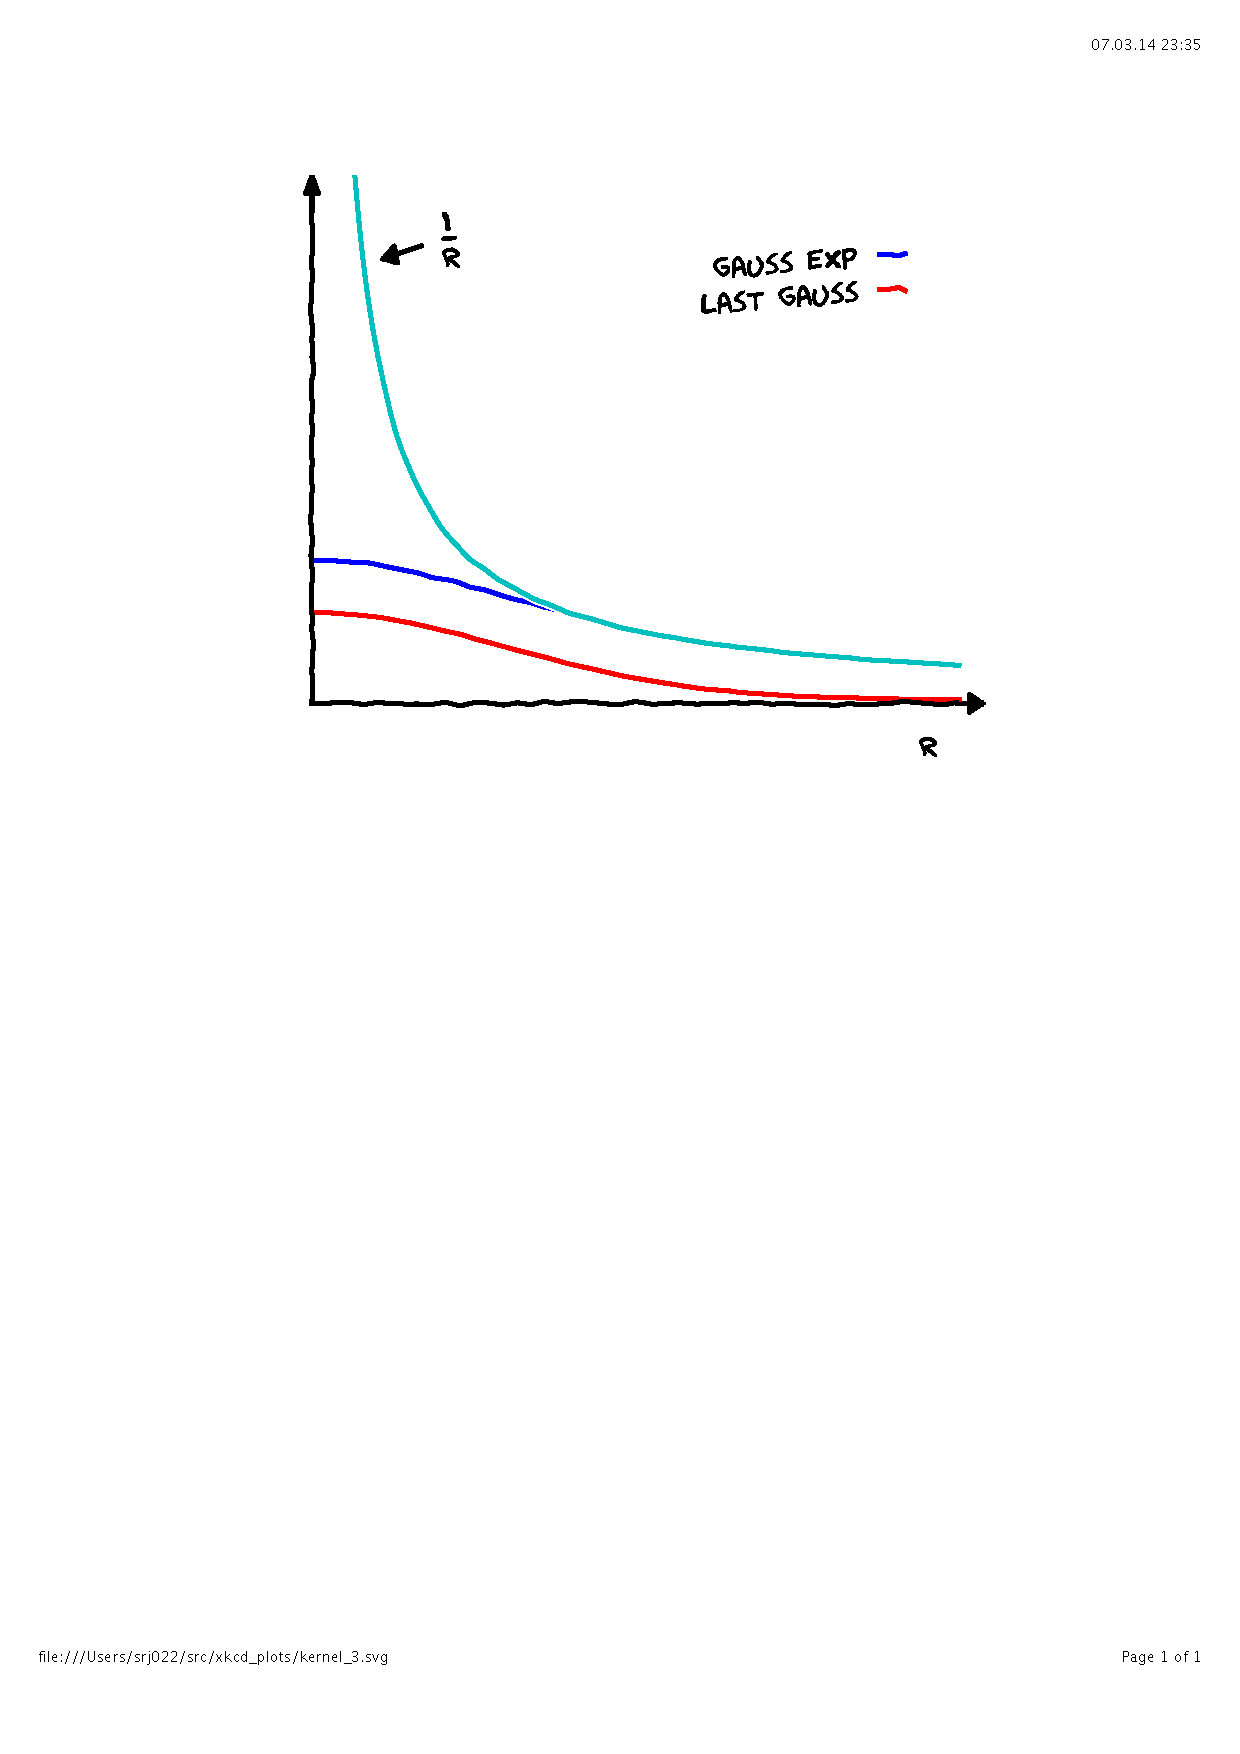
\includegraphics[scale=0.4, clip, viewport = 110 450 490 800] {figures/kernel_3.pdf}}
	\only<4>{\hspace{2mm}
        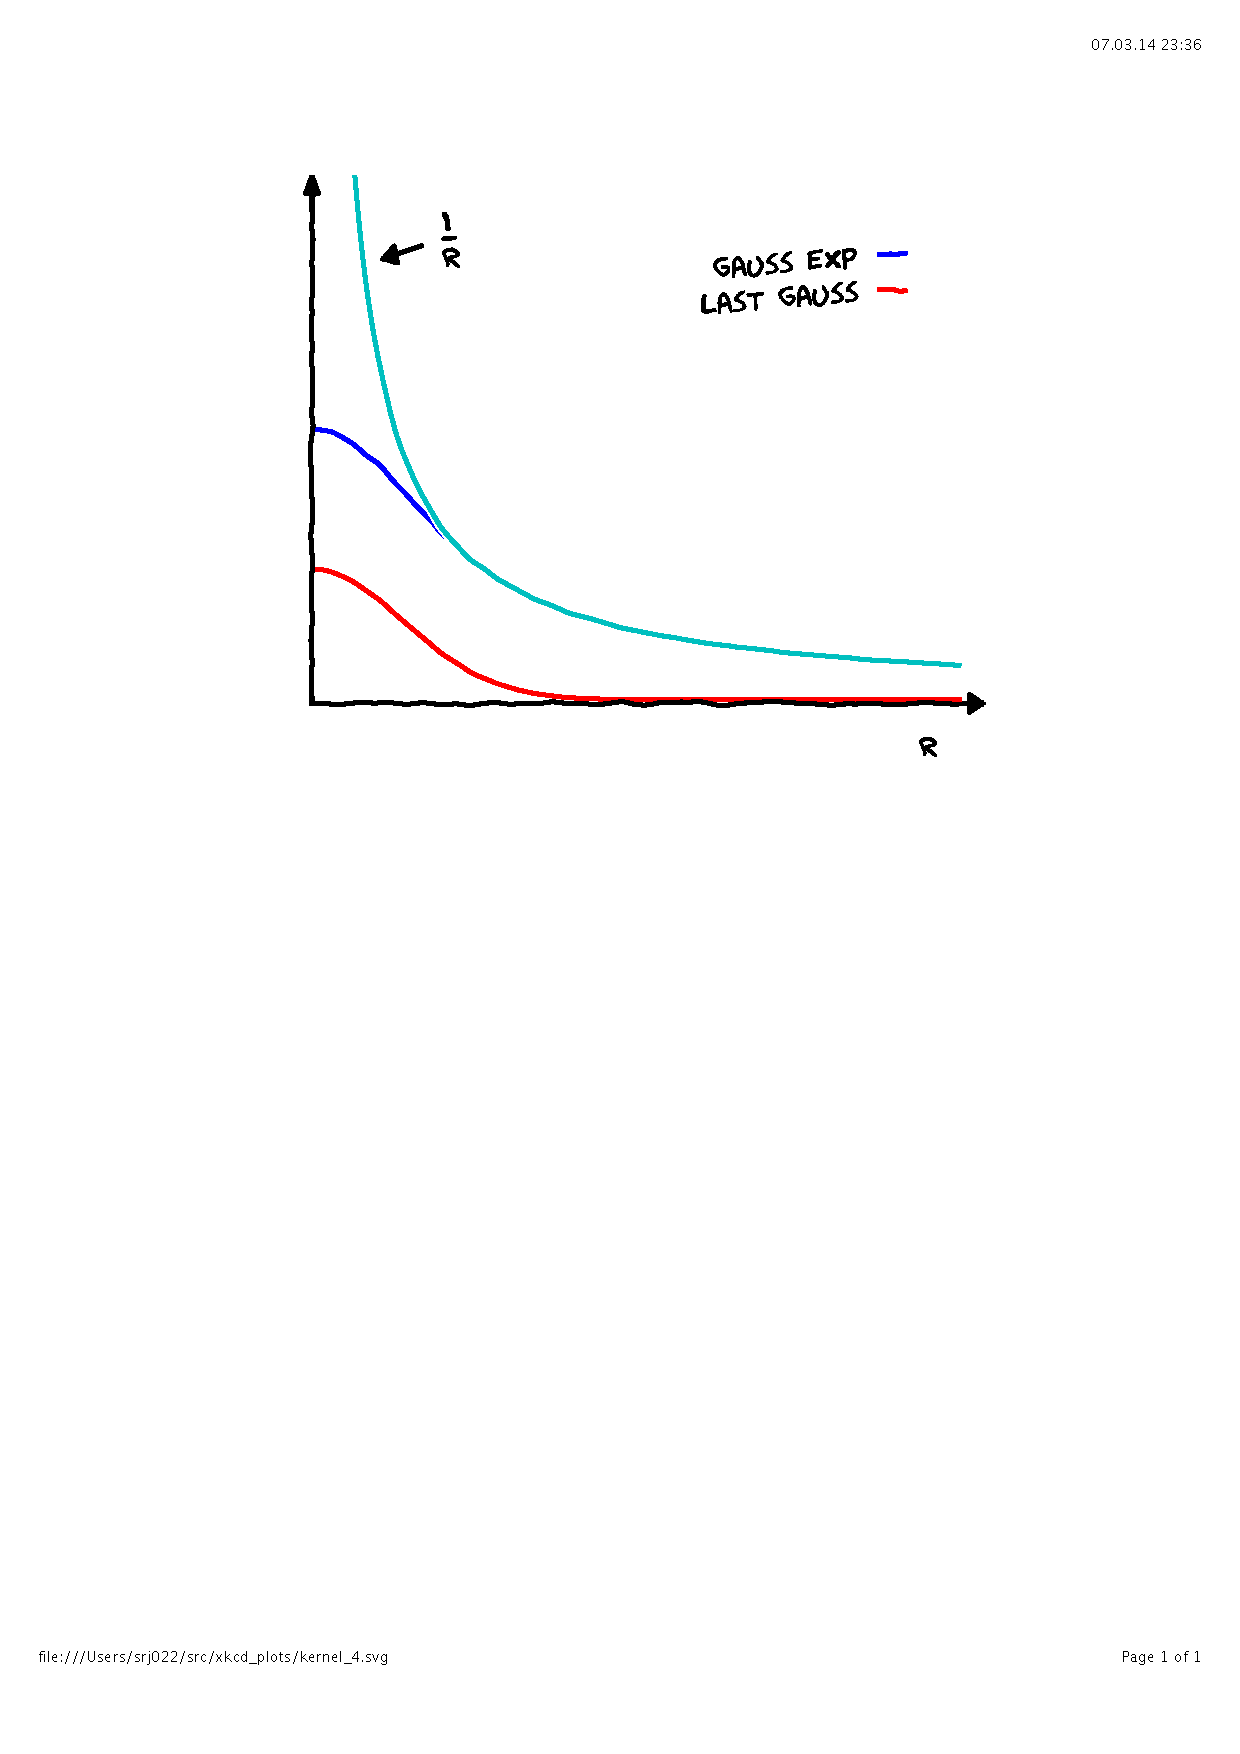
\includegraphics[scale=0.4, clip, viewport = 110 450 490 800] {figures/kernel_4.pdf}}
	\only<5>{\hspace{2mm}
        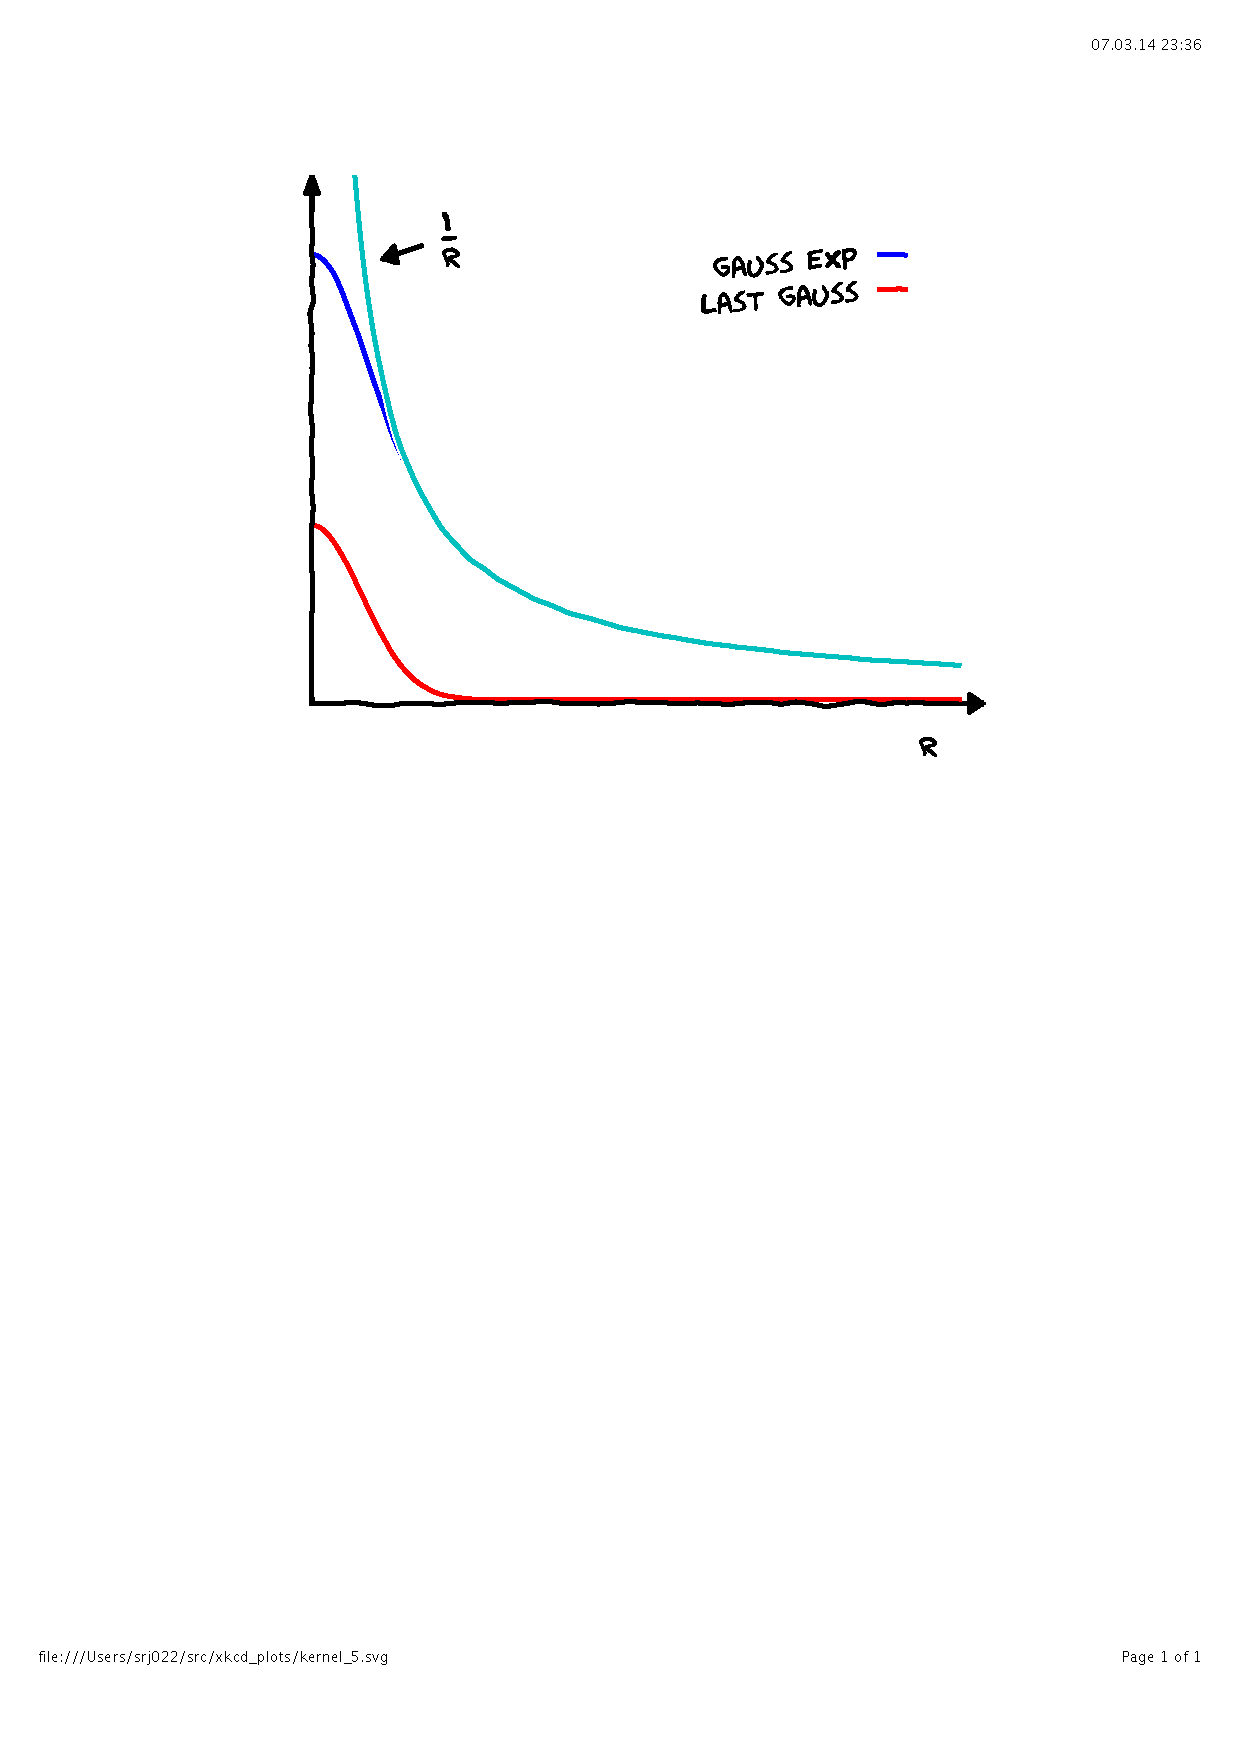
\includegraphics[scale=0.4, clip, viewport = 110 450 490 800] {figures/kernel_5.pdf}}
	\only<6>{\hspace{2mm}
        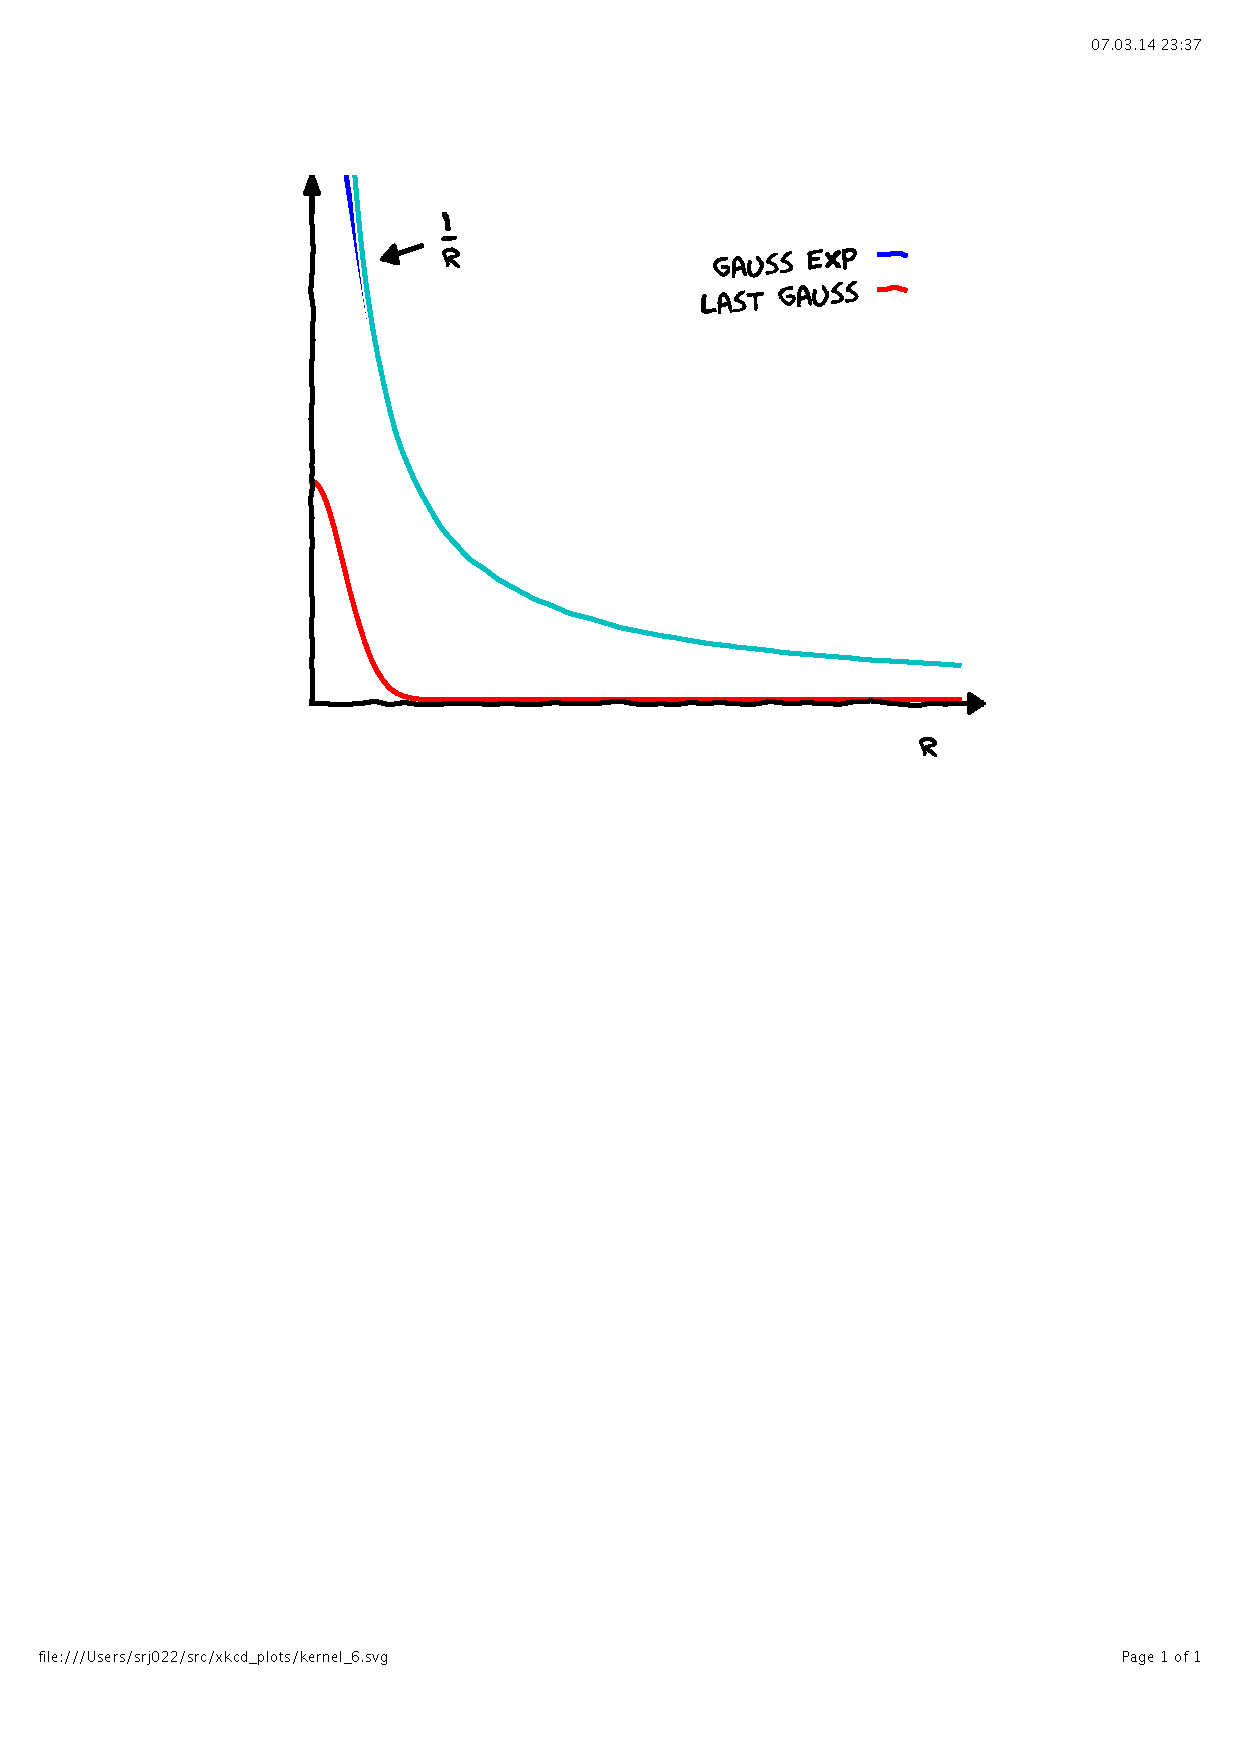
\includegraphics[scale=0.4, clip, viewport = 110 450 490 800] {figures/kernel_6.pdf}}
	\only<7>{\hspace{2mm}
        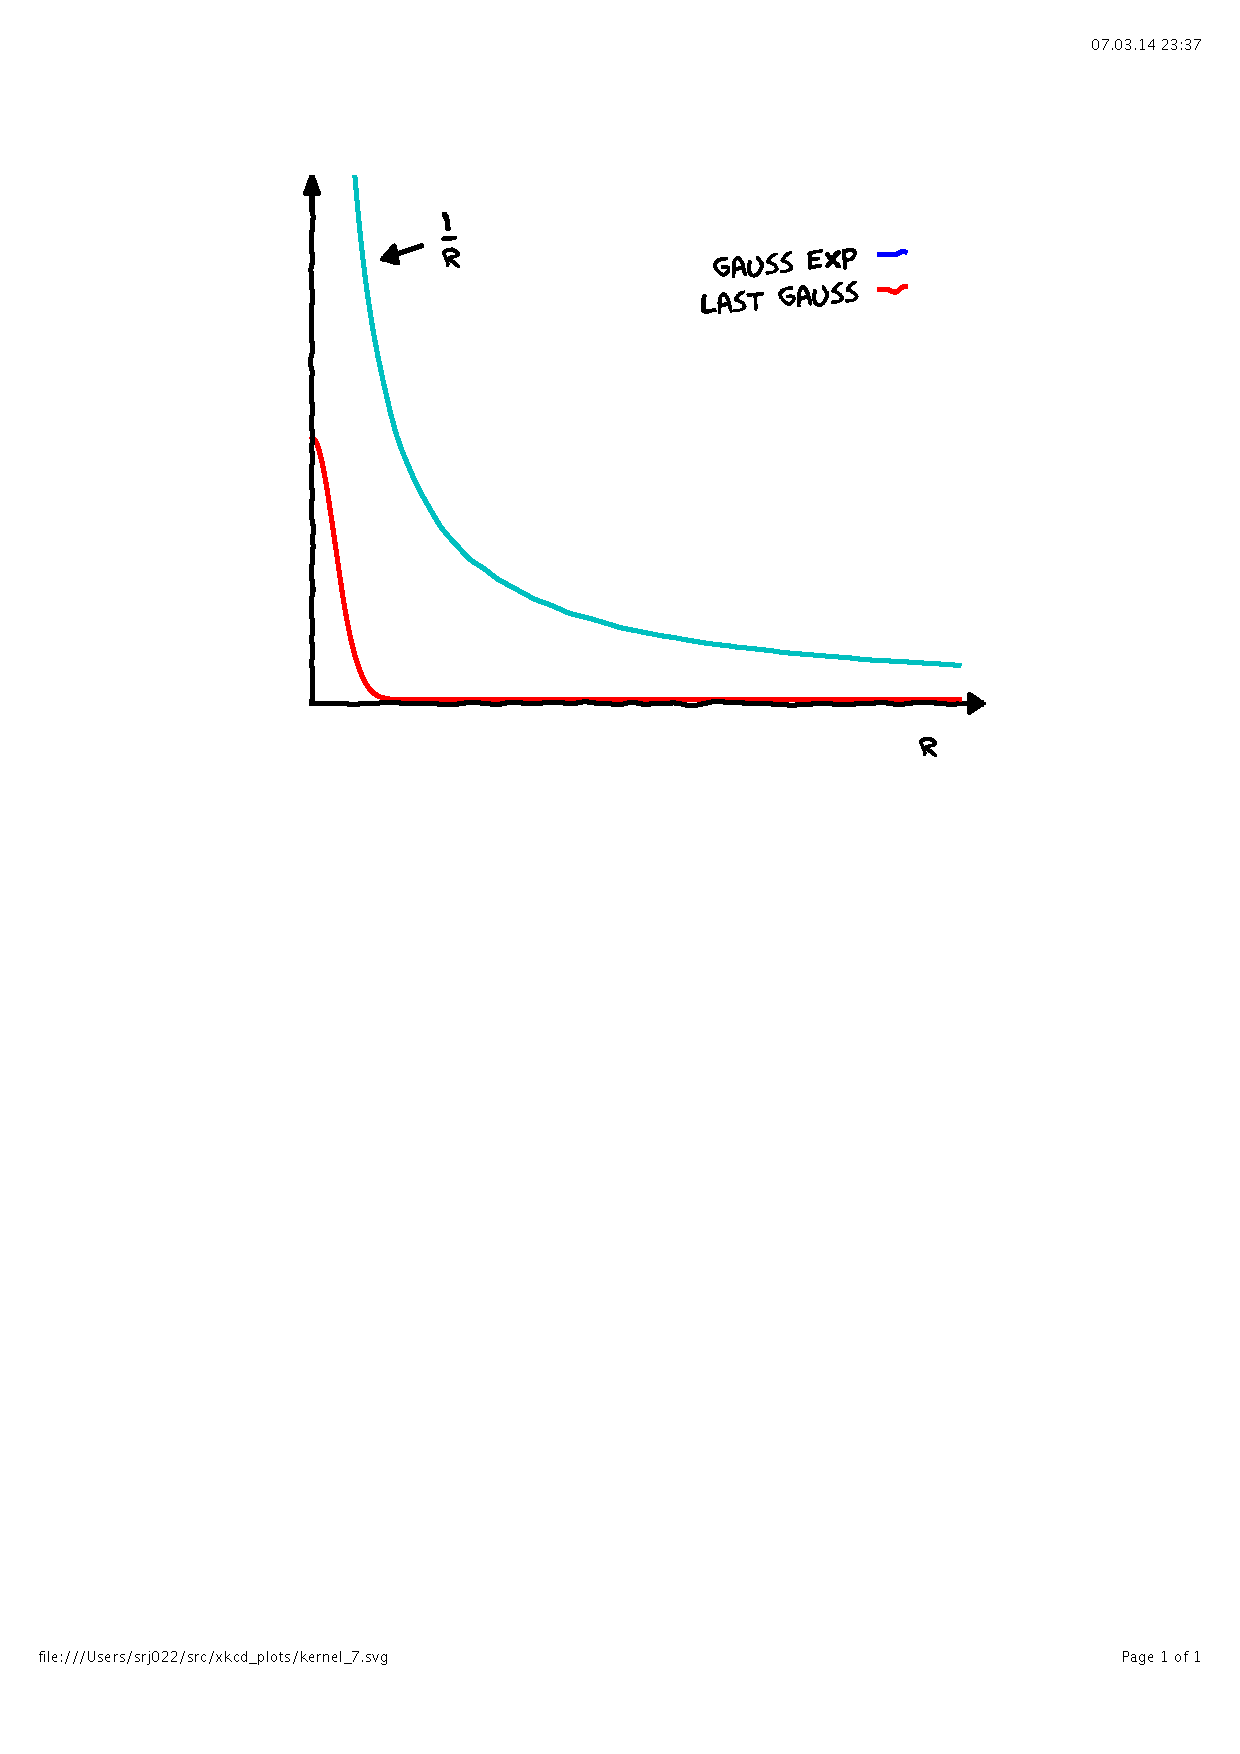
\includegraphics[scale=0.4, clip, viewport = 110 450 490 800] {figures/kernel_7.pdf}
        \vspace{0mm}}
	\only<8>{\hspace{0mm}
        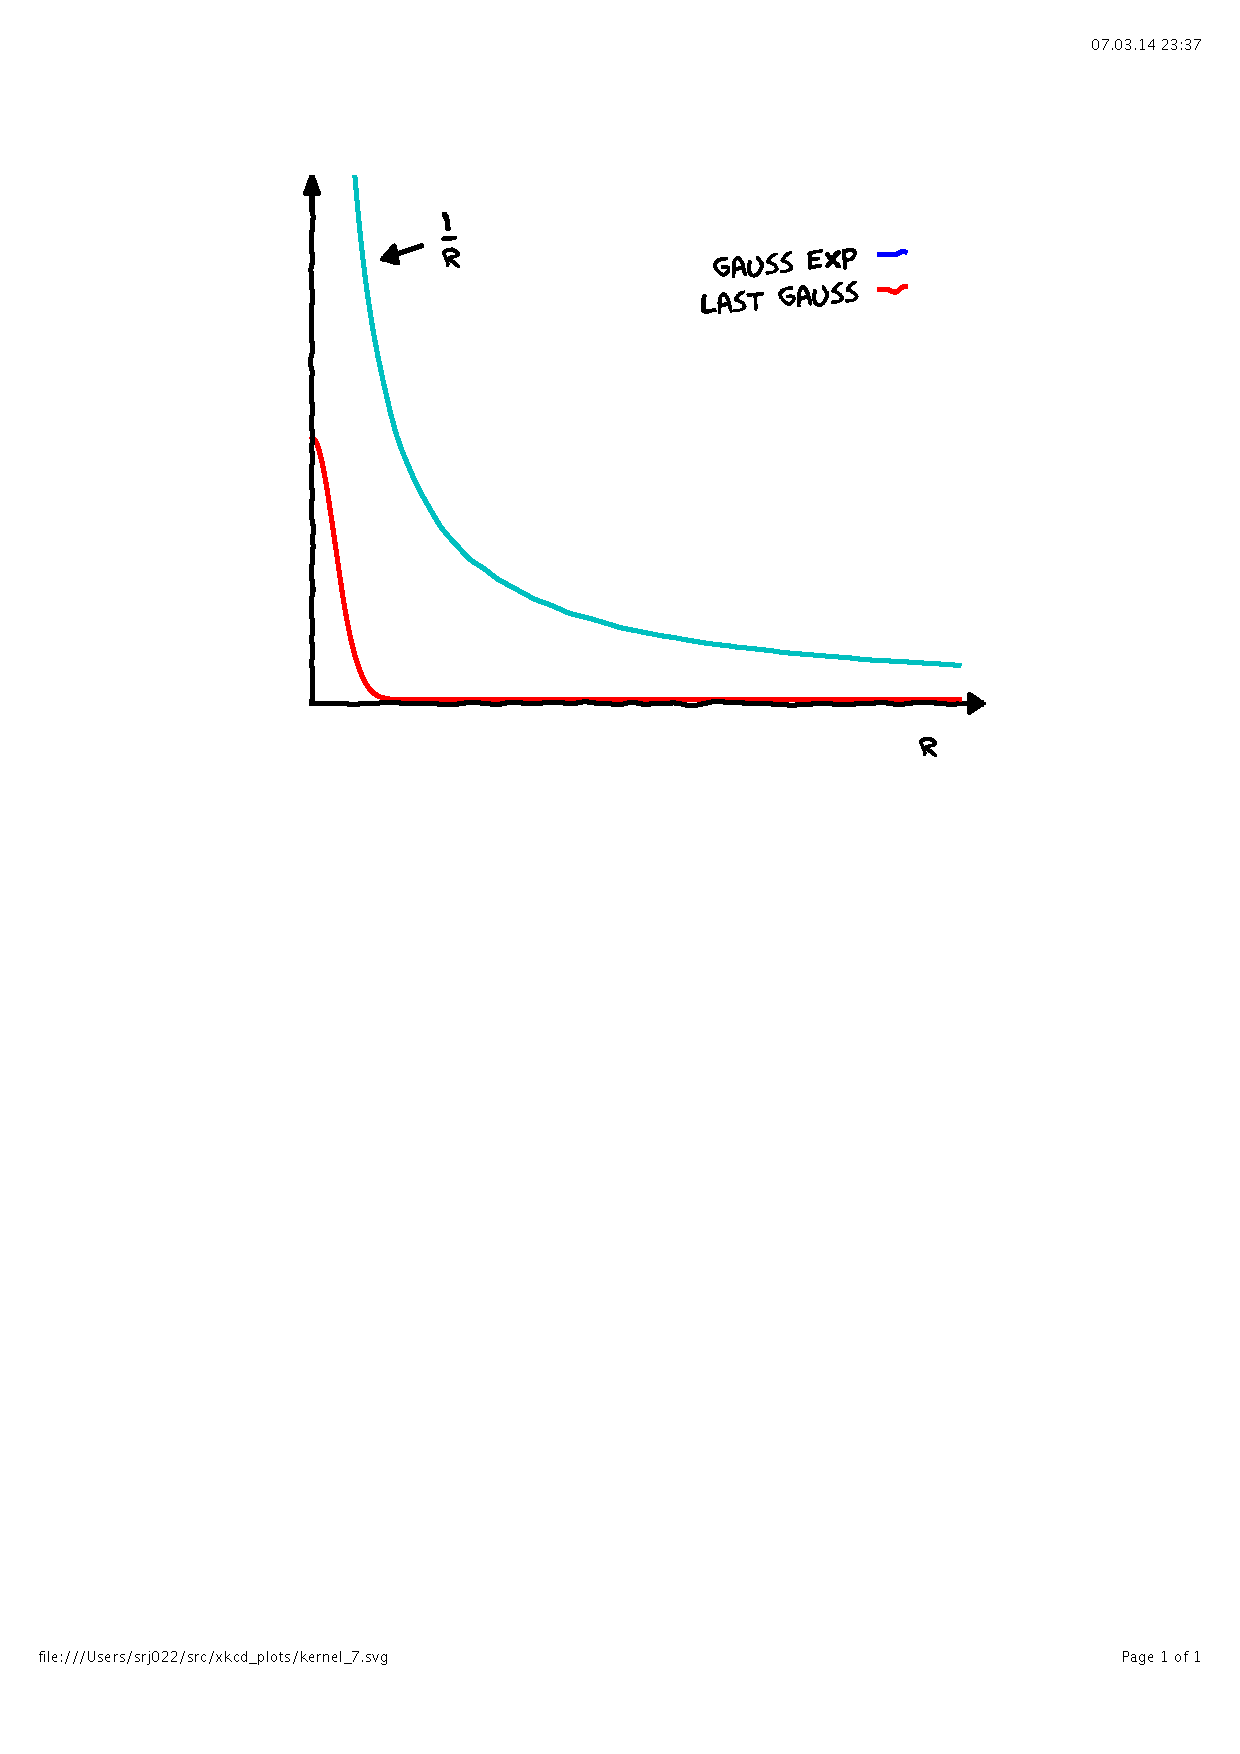
\includegraphics[scale=0.4, clip, viewport = 110 450 490 800] {figures/kernel_7.pdf}
        \vspace{3.5mm}}

        \only<9>{
        \centering
        \small{
        Combined with the \textbf{sparse}\\
        wavelet representation\\
        of operators we get\\
        \textbf{linear scaling algorithms!}}
        }
    \end{column}
    \end{columns}    

    \vspace{5mm}

    \centering
    \only<1,2,3,4,5,6,7,8,9>{\vspace{6mm}
    \tiny
    G. Beylkin, M.J. Mohlenkamp,
    {\it Proc. Nat. Acad. Sci.}
    \textbf{99(16)}
    (2002)
    }
\end{frame}


%\begin{frame}
%    \frametitle{Algorithm}
%    \tiny
%    \begin{algorithmic}[1]
%        \STATE create \tree skeleton of empty \nodes for the output function
%        \STATE create list of \emph{all} output \nodes
%        \WHILE{number of output \nodes in the current list $N>0$}
%            \FOR{each output \node in the current list}
%                \STATE fetch \emph{all} input \nodes within bandwidth of the \emph{full} operator
%                \STATE compute scaling and wavelet coefficients of output \node
%            \ENDFOR
%            \FOR{each \node of the output function}
%                \STATE remove \node from current list
%                \IF{\node needs to be refined}
%                    \STATE allocate children \nodes
%                    \STATE add children \nodes to the current list
%                \ENDIF
%            \ENDFOR
%        \ENDWHILE
%    \end{algorithmic}
%
%    \vspace{2mm}
%
%    \pause
%    \begin{algorithmic}[1]
%        \FOR{each separated component ($\kappa = 1,\dots,M$) of the operator}
%            \FOR{each s/w component of output function}
%                \FOR{each s/w component of input function}
%                    \STATE fetch appropriate operator component (e.g. $T\times A\times A$)
%                    \STATE construct bandwidth
%                    \STATE fetch input and operator \nodes within bandwidth
%                    \STATE prune list of input \nodes based on Cauchy-Schwartz screening
%                    \FOR{each contributing input \node}
%                        \STATE apply operator
%                    \ENDFOR
%                \ENDFOR
%            \ENDFOR
%        \ENDFOR         
%    \end{algorithmic}
%\end{frame}

%\begin{frame}
%    \frametitle{Linear scaling Coulomb interaction}
%    \scriptsize
%    \begin{columns}
%    \begin{column}{.10\textwidth}
%    \ \\
%    \end{column}
%    \begin{column}{.40\textwidth}
%	\centering
%
%        \vspace{2mm}
%	
%        \textbf{Alkane chains}
%	\begin{equation}
%	    \nonumber
%	    C_{n}H_{2n+2}, \qquad n=2,\dots,70
%	\end{equation}
%
%        \vspace{4mm}
%	
%        \textbf{Fitted curve}
%	\begin{equation}
%	    \nonumber
%	    t(n) = 12.5 + 2.34n^{0.754} 
%	\end{equation}
%    \end{column}
%    \begin{column}{.60\textwidth}
%	\centering
%
%        \vspace{3mm}
%
%	\begin{figure}
%	    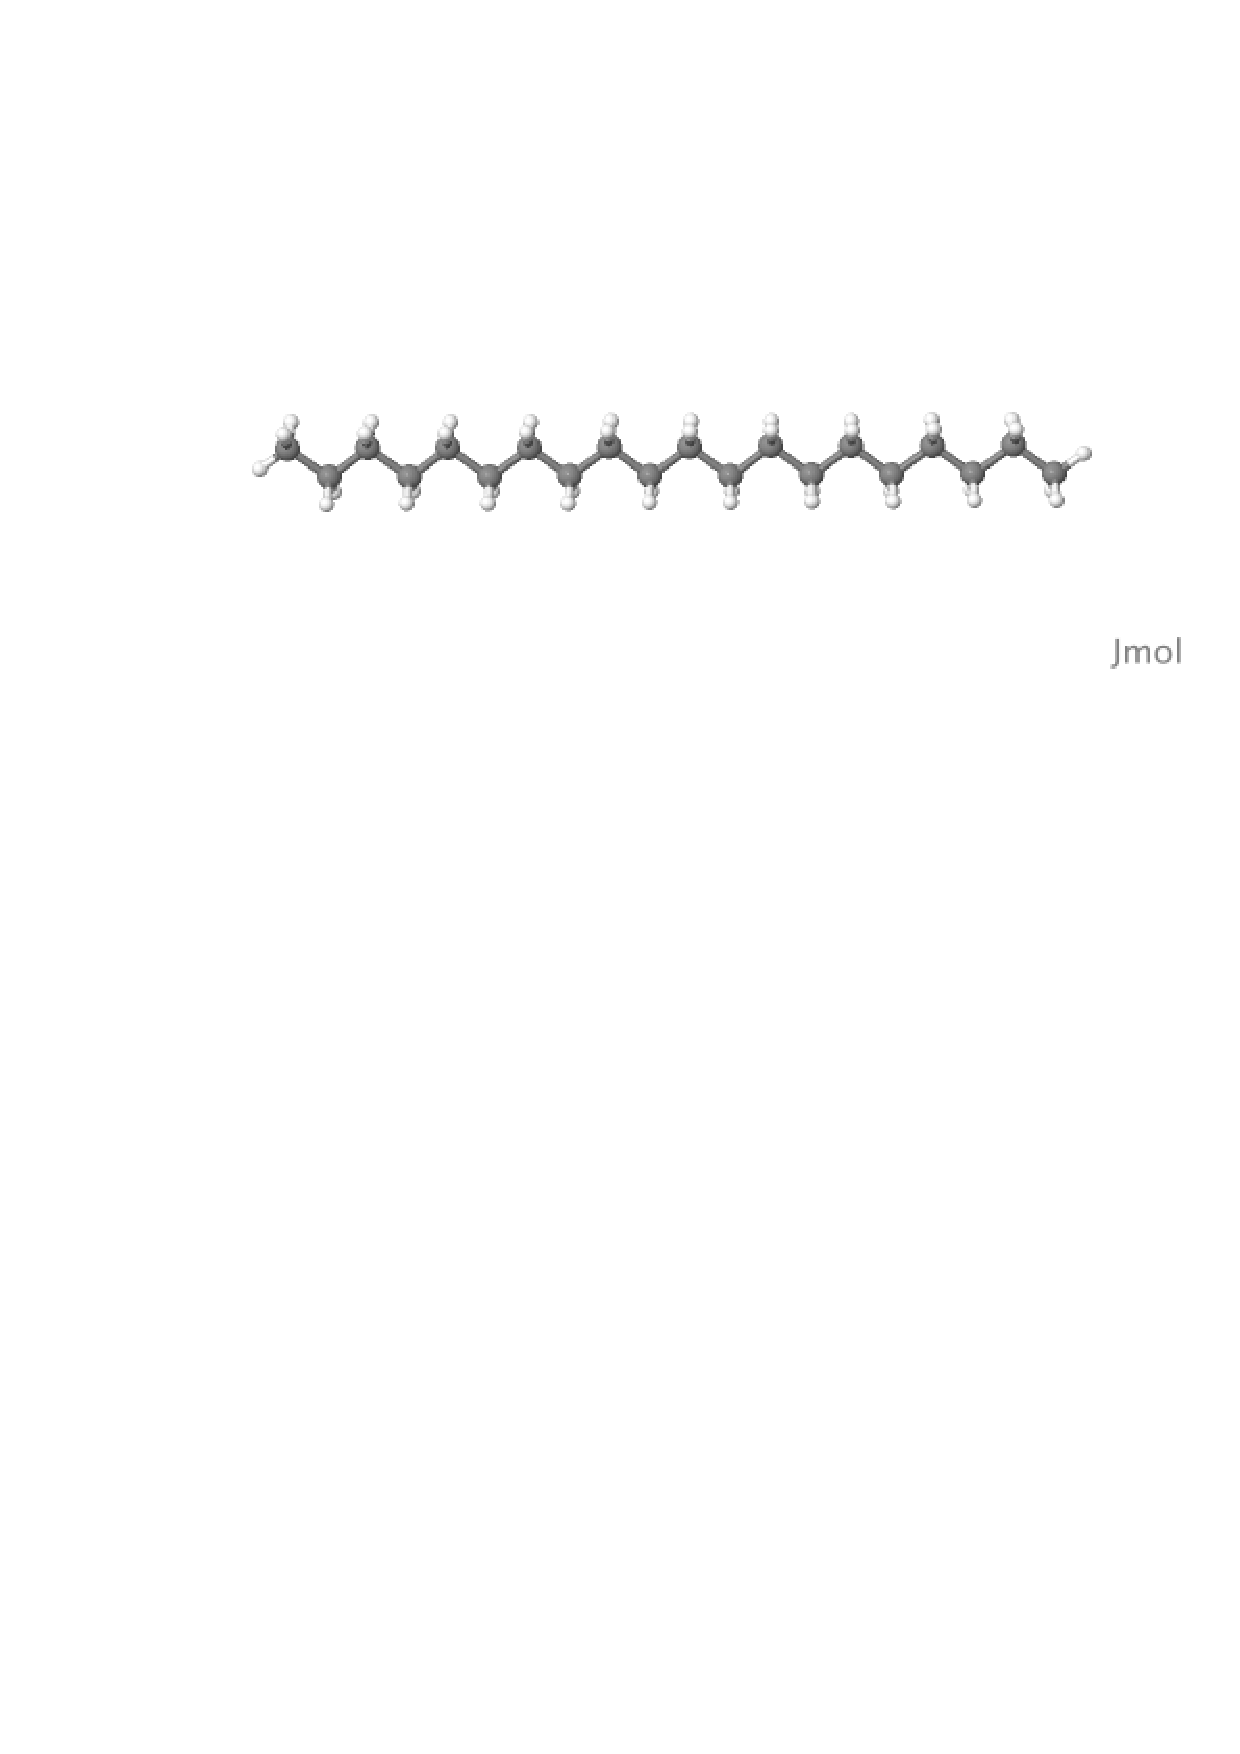
\includegraphics[scale=0.3, clip, viewport = 60 570 600 670]{figures/alkane.pdf}
%	\end{figure}
%
%        \vspace{2mm}
%
%	\textbf{Fitted curve}
%	\begin{equation}
%	    \nonumber
%	    t(n) = -6.0 + 1.33n^{0.991}
%	\end{equation}
%        \vspace{2mm}
%    \end{column}
%    \end{columns}    
%    \begin{center}
%	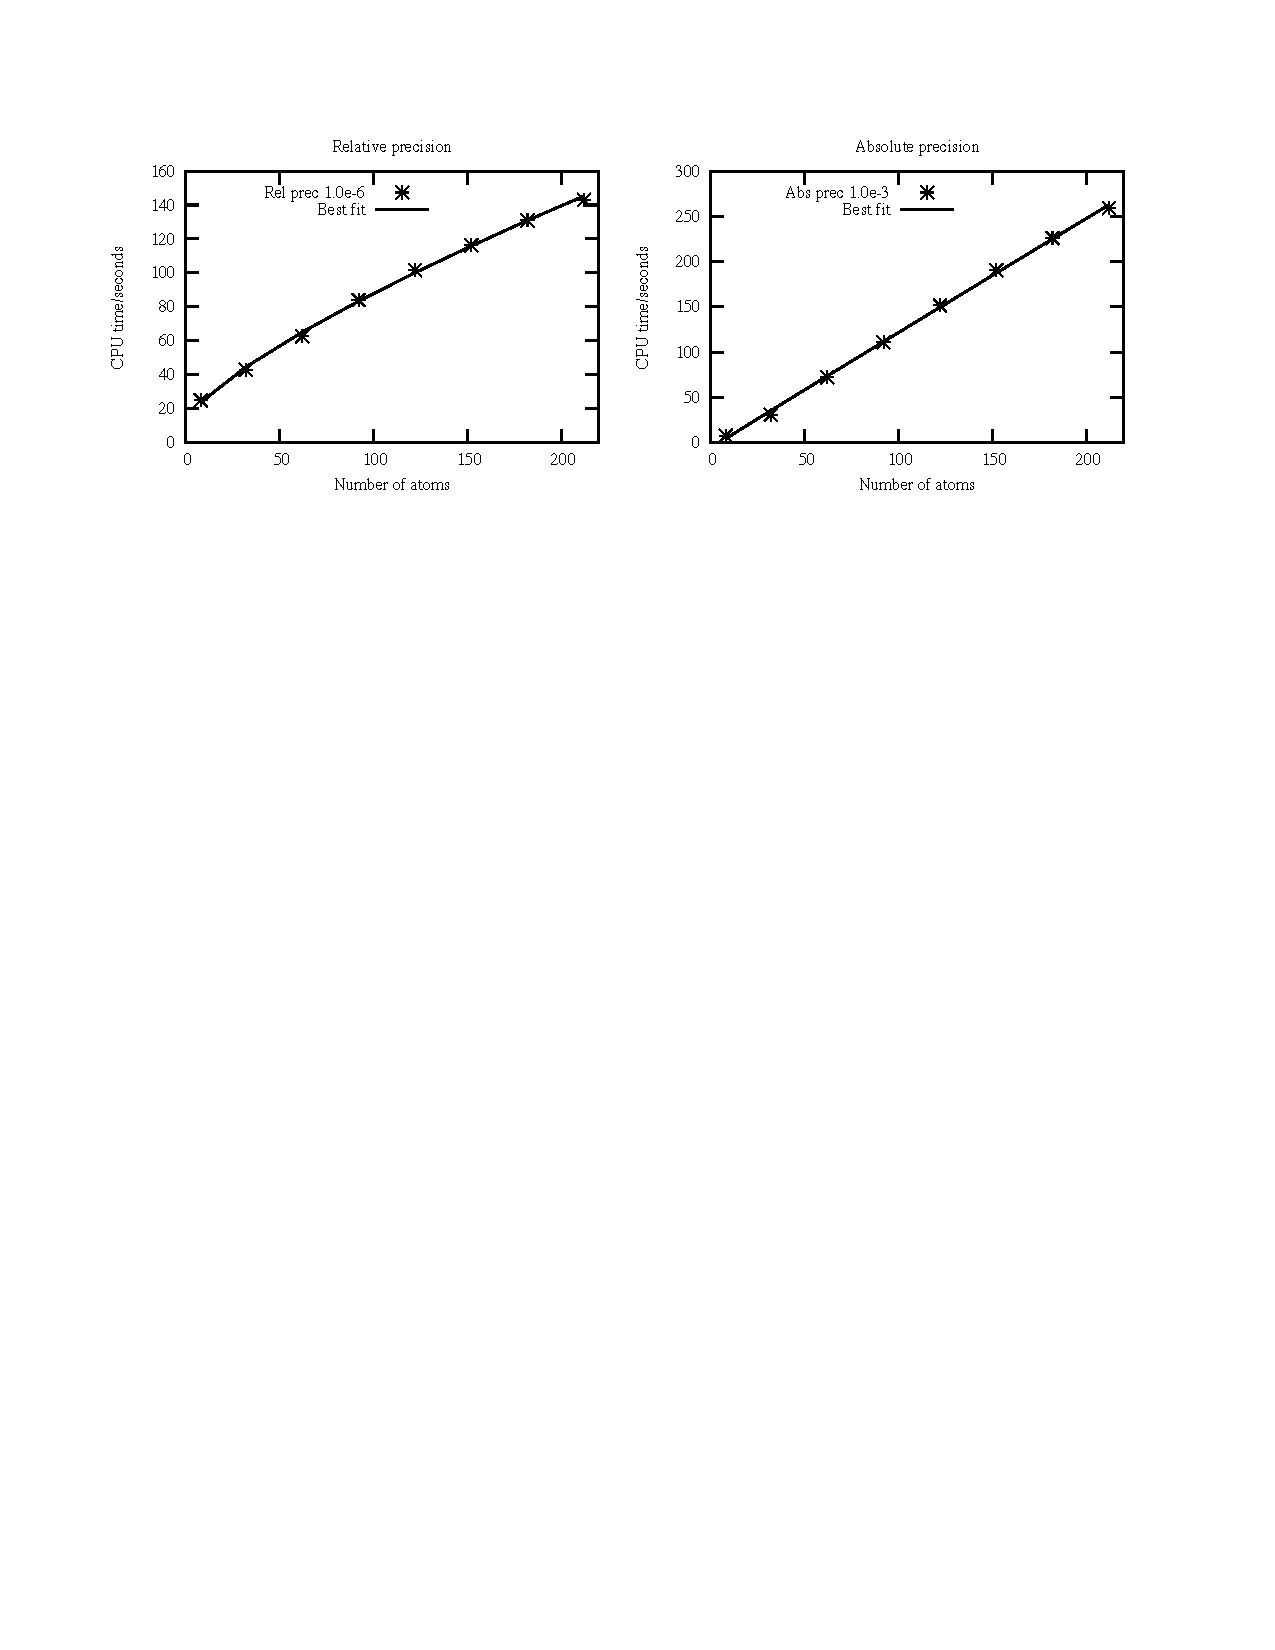
\includegraphics[scale=0.6, clip, viewport = 50 550 540 730]{figures/linearScaling.pdf}
%    \end{center}
%    \vspace{15mm}
%\end{frame}


